\documentclass[../body.tex]{subfiles}
\begin{document}
\subsection{Однослойный перцептрон}
\subsubsection{Линейная классификация}

\textit{Линейный классификатор} \cite{vorontsov} - один из самых простых алгоритмов классификации. Теория линейной классификации положила начало теории распознавания и стала источником базовых концепций, несмотря на ограниченность своего применения на практике.

В зависимости от количества разделяемых классов в рассматриваемой задаче получаем линейный классификатор в виде линейной (гиперплоскости) или кусочно-линейной поверхности.

Обучается такой классификатор путем подбора положения поверхности, соответствующего наилучшему разделению классов.
Аналогия линейного классификатора с нервной клеткой – его простейшее обоснование. Однако изначально подсмотренные у нейрофизиологии принципы обучения находят обоснование в математике.

Простейшим обоснованием линейного классификатора служит его аналогия с нервной клеткой - нейроном. Дальнейшее обобщение же идет по пути соединения простых элементов в сложные композиции, называемые уже искусственными нейронными сетями.

\subsubsection{Нейрофизиологическое обоснование линейного классификатора}

Рассмотрим упрощенный принцип работы нейрона - см рис. \ref{perceptronBioNeuron}. Будем смотреть на него, как на устройство, которое на каждом такте своей работы принимает заряды от множества входов-дендритов, и если суммарный накопленный заряд превосходит некоторый порог, передает импульс через множество выходов-синапсов. Связанные друг с другом нейроны, распространяющие направленные волны импульсов, образуют нервную систему. 

Математическая модель нейрона упрощает эту уже упрощенную модель нейрона биологического, что совершенно нормально, потому как теория искусственных нейронных сетей и не ставила перед собой задачи воспроизведения функционирования биологической нейронной сети.

\begin{figure}[H]
	\center{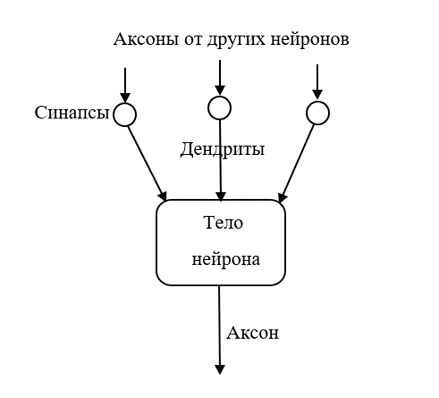
\includegraphics[width=.6\textwidth]{img/bioneuron.png}}
	\caption{Упрощённая схема работы биологического нейрона}
	\label{perceptronBioNeuron}
\end{figure}

Будем использовать математическую модель нейрона, известную как модель МакКаллока-Питтса - рис. \ref{perceptronNeuronModel}.

\textit{Модель МакКаллока–Питтса (1943):}  Пусть $X$ - пространство объектов; $Y$ - множество допустимых ответов; объекты описываются $n$ числовыми признаками $f_j: X \rightarrow \mathds{R}, j = 1,...,n$. Вектор $x = (x_1,... ,x_n)\in \mathds{R}^n$, где $x^j = f_j(x)$, называется признаковым описанием объекта $x$.

\begin{figure}[H]
	\center{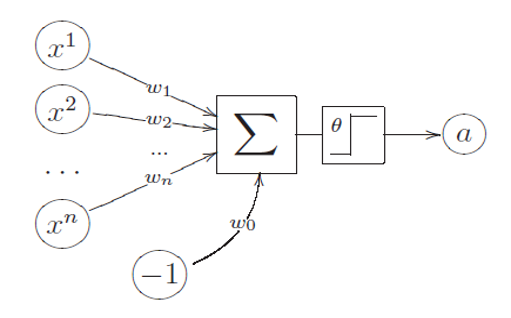
\includegraphics[width=.7\textwidth]{img/McCullochPittsNeuron.png}}
	\caption{Модель МакКаллока-Питса (графическая трактовка)}
	\label{perceptronNeuronModel}
\end{figure}

Полагаем все признаки и ответы бинарными $(Y = {0, 1})$. Значения признаков $x^j = f_j(x)$ трактуем как величины импульсов, поступающих на вход нейрона через n входных синапсов. Поступающие на вход синапсы складываются с весами $w_1, ..., w_n$. Знак $j$-ого веса определяет будет ли $j$-ый синапс возбуждающим или тормозящим. При превышении суммарным импульсом порога активации $w_0$ нейрон возбуждается и выдает вход $1$, иначе выдается $0$. Таким образом, получаем, что нейрон вычисляет $n$-арную булеву функцию вида $a(x) = \varphi(\sum_{j=1}^{n} w_j x^j - w_0)$, где $\varphi(z) = [z \geq 0]$ - пороговая функция Хевисайда. Функция $\varphi$, преобразующая значение суммарного импульса во входное значение нейрона, принято называть функцией активации.

Запишем линейную модель нейрона через скалярное произведение:
$$a(x, w) = \varphi(\sum_{j=1}^{n} w_j x^j) = \varphi(<w, x>), w = (w_0, ..., w_n)^T, x = (x^0, ..., x^n)^T$$.

Модель нейрона по МакКаллоку-Питтсу представляет собой линейный пороговый классификатор. Эта модель может быть обобщена на случай произвольных вещественных входов и выходов и произвольных функций активации, в том числе и на сигмоидную функцию, о которой речь пойдет в главе, посвященной логистической регрессии.

\subsubsection{Обучение градиентным методом}

$y^*: X\rightarrow Y$ - целевая зависимость, известная только на объектах обучающей выборки $X^l = (x_i, y_i)_{i=1}^{l}, y_i = y^*(x_i)$.
Задача состоит в нахождении вектора весов $w$ такого, что $a(x, w)$ аппроксимирует целевую зависимость $y^{*}$. Таким образом, ищем вектор $w$, доставляющий минимум функционалу:
$$Q(w) = \sum_{i=1}^{l}\mathcal{L}(a(x_i, w), y_i)\rightarrow min.$$ Тут $\mathcal{L}(a, y)$ - заданная функция потерь, характеризующая величину ошибки ответа $a$ при правильном ответе $y$. Рассмотрим задачу минимизации в общем случае, пока не конкретизируя функцию $\mathcal{L}(a, y)$.
Применим для минимизации $Q(w)$ метод градиентного спуска (см. 2.1). Выбирается некоторое начальное приближение для вектора весов $w$ и запускается итерационный процесс, на каждом шаге которого вектор $w$ изменяется в направлении наиболее быстрого убывания функционала $Q(w)$. Это направление противоположно вектору градиента $\nabla Q(w) = (\frac{\partial Q(w)}{\partial w_j})_{j=1}^n: w := w - \eta\nabla Q(w)$, где $\eta > 0$ - величина шага в направлении антиградиента, называемая также темпом обучения.
Предполагаем, что $\mathcal{L}$ и $\varphi$ дифференцируемы, распишем градиент:
$$w := \eta\sum_{i=1}^{l}\mathcal{L}_a^{'}(a(x_i, w), y_i)\varphi^{'}(<w, x_i>)x_i.$$

\SetKwRepeat{Do}{do}{while}
\begin{algorithm}[H]
	\KwData{$X^l$ - обучающая выборкаб $\eta$ - темп обучения, $\lambda$ - параметр сглаживания функционала $Q$}
	\KwResult{синаптические веса $w_0, ..., w_n$}
	инициализация веса $w_j, j = 1, ..., n$\;
	инициализация текущей оценки функционала $Q(w) := \sum_{i=1}^l\mathcal{L}(a(x_i, w), y_i)$\;
	\Do{занчение $Q$ не стабилизируется и/или веса $w$ не перестанут меняться}{
		взять случайный $x_i \in X^l$ и вычислить выход $a(x_i, w)$ и ошибку $\varepsilon_i := \mathcal{L}(a(x_i, w), y_i)$\;
		сделать шаг градиентного спуска: $w := w - \eta\mathcal{L}_a^{'}(a(x_i, w), y_i)\varphi^{'}(<w, x_i>)x_i$\;
		оценить значение функционала $Q := ((1 - \lambda)Q+ \lambda\varepsilon_i)$\;
	}
	\caption{Обучение перцептрона градиентным методом}
\end{algorithm}


\subsubsection{Однослойный перцептрон Розенблатта}

Во второй половине 20-ого века Розенблатт предложил эвристический алгоритм обучения нейрона \cite{rosenblatt} \cite{vorontsov}, основанный на принципах нейрофизиологии, экспериментально обнаружив, что синхронное возбуждение связанных нервных клеток усиливает синаптическую связь между ними. И чем чаще синапс угадывает правильный ответ, тем сильнее становится связь. Такая тренировка связи приводит к постепенному запоминанию информации. Связь ослабевает, если синапс начинает часто ошибаться или вообще перестаёт использоваться, информация начинает забываться. Так память реализуется в синапсах. В математической модели нейрона роль памяти играет вектор синаптических весов $w$. 
Данное правило обучения нетрудно формализовать. Как признаки, так и ответы будем пока полагать бинарными. Перед началом обучения вектор весов некоторым способом инициализируется, например, заполняется нулевыми или случайными значениями. Затем обучающие объекты  $x_i$ по очереди подаются на вход модели МакКаллока–Питтса, и выданные ответы сравниваются с правильными.

Если ответ $a(x_i)$ совпадает с $y_i$, то вектор весов не изменяется.
Если  $a(x_i) = 0$ и $y_i = 1$, то вектор весов $w$ увеличивается. Увеличивать имеет смысл только те веса $w_j$, для которых $x_i^j \neq 0$; изменение других компонент не повлияет на результат. Положим $w := w + \eta x_i$, где $\eta > 0$ - темп обучения.
Если $a(x_i) = 1$ и $y_i = 0$, то вектор весов уменьшается:  $w := w - \eta x_i$.
Поскольку все величины бинарные, три случая объединяются в одну формулу:
\begin{equation*}
	w := 
	\begin{cases}
		w &\text{if $a(x_i) = y_i$}\\
		w + \eta x_i &\text{$a(x_i) = 0$ and $y_i = 1$}\\
		w - \eta x_i &\text{$a(x_i) = 1$ and $y_i = 0$}
	\end{cases}
\end{equation*}
$$w := w - \eta(a(x_i) -  y_i)(*)$$

Обучающие объекты пропускаются через это правило многократно, пока веса изменяются. Этот алгоритм обучения и есть \textit{однослойный перцептрон Розенблатта}.
Перцептрон можно, помимо того, обучать градиентным спуском. 
Формализуем рассматриваемую задачу: $\exists {(x_i, \widetilde{y_i})}_{i=1,...,m}, x_i \in \mathds{R}^N, y_i \in \mathds{R}^1$ - тренировочные экхемпляры, $w$ - вектор параметров(весов), $w \in \mathds{R}^{N+1}$.
Покажем, что градиентный спуск всегда будет сходиться, если взять квадратичную функцию стоимости.
$J(w) = \frac{1}{2m}\sum_{i=1}^m (w\widetilde{x_i} - \widetilde{y_i})^2 \rightarrow min$, $y_i$ - гипотеза перцептрона, вычисляемая по формуле $y_i(\widetilde{x_i}) = heaviside(w \widetilde{x_i})$, где $\widetilde{x_i} = (1, x_i)^T$.
Рассмотрим компоненты градиента: $$\frac{\partial J}{\partial w_j} = \frac{\sum_{i=1}^m (w\widetilde{x_i} - \widetilde{y_i})x_{ij}}{m}.$$
Рассмотрим вклад от отдного тренировочного экземпляра, а не усредненное по количеству тренируемых данных:
$$\frac{\partial J_i}{\partial w_j} = (w \widetilde{x_i} - \widetilde{y_i})x_{ij}.$$Производная этой функции непрерывна и ограничена на всем пространстве параметров: $$\frac{\partial^2 J_i}{\partial w_j^2} = (1, x_i)_j x_{ij} = x_{ij}^2.$$
По лемме о липшицевости \cite{lizorkin} $\exists$ константа липшица для градиента.
Пусть $L_i = max(x_{ij}^2)$ по j - константа Липшица для вклада одного тренировочного экземпляра. $L := \sum_{i=1}^m L_i$.
Если градиент подчиняется условию Липшица, то метод градиентного спуска непременно будет сходиться к $min$. 
Таким образом, обосновано примнение градиентного спуска для обучения перцептрона с данной функцийей стоимости.
 

\subsubsection{Пример обучения перцептрона}

У нас есть набор обучающих данных - результаты двух экзаменов (источник: \url{https://coursera.org/learn/machine-learning/}). Если оба экзамена сданы, то точка (студент, сдававший экзамены) попадает в положительный класс, если же его баллы ниже определённого порога, то в другой. Ставится задача разделения этих двух классов.
Результат обучения перцептрона показан на рис.\ref{perceptronOutput}. С найденными при обучении весами функция потерь $J = 0.12$.

\begin{figure}[H]
	\center{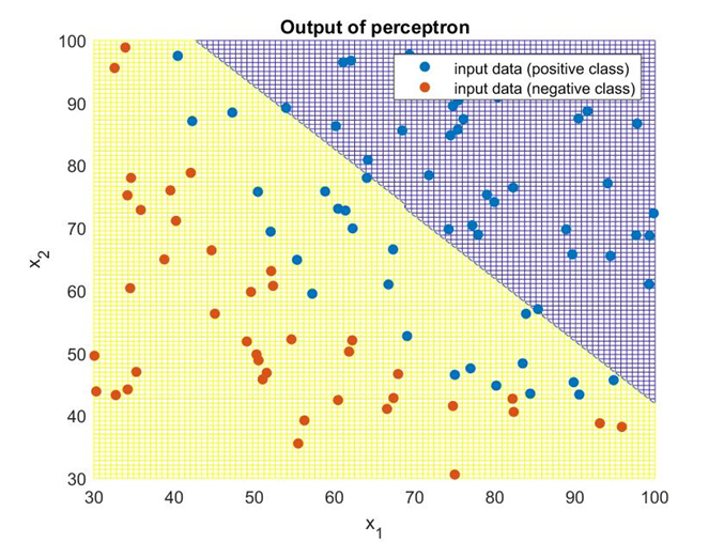
\includegraphics[width=.85\textwidth]{img/perceptronOutput.png}}
	\caption{Граница, формируемая перцептроном после обучения}
	\label{perceptronOutput}
\end{figure}

\end{document}